% !TEX program = xelatex
% Compile: xelatex report.tex (twice for TOC/refs)

\documentclass[12pt, a4paper, UTF8]{ctexart}

% ---- packages ----
\usepackage[margin=2.5cm]{geometry}
\usepackage{graphicx}
\usepackage{xcolor}
\usepackage{hyperref}
\usepackage{listings}
\usepackage{amsmath}
\usepackage{amssymb}
\usepackage{booktabs}
\usepackage{multirow}
\usepackage{enumitem}
\usepackage{tikz}
\usetikzlibrary{positioning, shapes.geometric, arrows.meta, fit, calc}
\usepackage{fancyhdr}
\usepackage{titlesec}

% ---- hyperref ----
\hypersetup{
  colorlinks=true,
  linkcolor=blue!60!black,
  urlcolor=blue!60!black,
  citecolor=blue!60!black,
  pdftitle={基于 Newton 物理引擎与 Claude VLA 的具身智能交互演示},
  pdfauthor={kingcode},
}

% ---- listings ----
\definecolor{codebg}{rgb}{0.96, 0.96, 0.96}
\definecolor{codekey}{rgb}{0.10, 0.30, 0.70}
\definecolor{codecmt}{rgb}{0.40, 0.55, 0.40}
\definecolor{codestr}{rgb}{0.65, 0.35, 0.10}
\lstset{
  language=Python,
  backgroundcolor=\color{codebg},
  basicstyle=\ttfamily\footnotesize,
  keywordstyle=\color{codekey}\bfseries,
  commentstyle=\color{codecmt}\itshape,
  stringstyle=\color{codestr},
  showstringspaces=false,
  breaklines=true,
  frame=single,
  framerule=0.3pt,
  rulecolor=\color{black!20},
  numbers=left,
  numberstyle=\tiny\color{gray},
  numbersep=8pt,
  xleftmargin=2em,
  tabsize=4,
}

% ---- titlesec ----
\titleformat{\section}{\large\bfseries}{\thesection}{0.6em}{}
\titleformat{\subsection}{\normalsize\bfseries}{\thesubsection}{0.5em}{}

% ---- headers ----
\pagestyle{fancy}
\fancyhf{}
\fancyhead[L]{\small Newton VLA 课堂演示 — 设计报告}
\fancyhead[R]{\small\thepage}
\renewcommand{\headrulewidth}{0.4pt}

% ---- title ----
\title{\textbf{\Large 基于 Newton 物理引擎与 Claude VLA \\的具身智能交互演示}\\[6pt]
       \large 设计报告}
\author{kingcode}
\date{2026 年 5 月}

\begin{document}
\maketitle

% ============================================================
\begin{abstract}
\noindent
本项目实现了一个 3 分钟课堂级具身智能交互演示，运行在一台
苹果芯片的 MacBook 上，无需 GPU 或云端推理。系统结合 NVIDIA
Newton XPBD 物理引擎、pygame 二维渲染管线，以及 Claude
命令行客户端作为视觉--语言--动作 (VLA) 解析器，提供三种
交互模式：基于模型预测控制 (MPC) 的接球，自然语言驱动的
抓取与堆叠，以及四种装饰性手势 (wave / point / bow / dance)。
工业模式额外引入第二只固定底座机械臂，自主循环搬运专属工件，
形成双臂并行的工厂调度视觉效果。核心技术贡献包括：
(1) 闭式弹道求解的轻量 MPC；
(2) 关键词预飞 + Claude 精化的混合 VLA 解析管线，
将平均命令到动作延迟从 9.4 s 压缩到 1 ms；
(3) 固定臂与移动臂共享 \texttt{world.blocks} 但物理无冲突的
执行器抽象。系统经 214 项单元与集成测试覆盖，实战演示中
接球命中率 62\%--82\%，VLA 链路稳定跑通 ``pizza tower
\(\to\) stack red green blue'' 等模糊语义指令。

\medskip
\noindent\textbf{关键词：}\quad 具身智能、模型预测控制、
视觉--语言--动作模型、物理仿真、人机交互
\end{abstract}

% ============================================================
\tableofcontents
\newpage

% ============================================================
\section{引言}

\subsection{项目背景与动机}
具身智能 (Embodied AI) 是当前人工智能领域最具张力的方向之一：
大语言模型已经能像人类一样写代码、答题、规划，但 ``身体''
仍然是缺失的最后一公里。在课堂教学场景中，学生很难直观感受
``经典控制''与``学习驱动''之间的分野，也难以亲手验证大语言
模型在闭环物理世界中的实际表现。本项目以一台 MacBook 为
硬件平台、以 Newton 物理引擎为仿真后端、以 Claude 为 VLA
大脑，搭建一个 3 分钟即可完整呈现的现场演示，目的是让观众
在不到一节课的时间内同时体验：
\begin{itemize}[leftmargin=*, itemsep=0pt]
  \item 经典控制 (MPC) 的精确性与可预测性；
  \item 自然语言到结构化动作的端到端解析；
  \item 大模型推理延迟与降级策略的工程取舍；
  \item 多臂协同与并行任务的视觉效果。
\end{itemize}

\subsection{设计目标}
\begin{enumerate}[leftmargin=*]
  \item \textbf{现场稳定}：3 分钟完整流程不允许出现死机、
    NaN、模型超时等致命异常；
  \item \textbf{零云依赖}：所有推理、物理、渲染本地化，
    无需保证网络；
  \item \textbf{60 fps 视觉}：1920\,$\times$\,1080 全屏渲染
    平均帧率不低于 58 fps；
  \item \textbf{毫秒级首响应}：观众输入命令后机械臂在 1 ms
    内开始动作；
  \item \textbf{可测试}：所有关键路径（物理、控制、解析、
    渲染）必须有自动化回归测试。
\end{enumerate}

\subsection{报告组织}
第 \ref{sec:tech} 节介绍背景技术；第 \ref{sec:arch} 节展示
系统总体架构与模块划分；第 \ref{sec:algo} 节阐述核心算法
（接球 MPC、IK、缓动函数、混合 VLA 管线）；第 \ref{sec:impl}
节聚焦实现细节与工程取舍；第 \ref{sec:eval} 节给出测试覆盖
与性能基准；第 \ref{sec:conclusion} 节总结与展望。

% ============================================================
\section{相关技术}\label{sec:tech}

\subsection{NVIDIA Newton XPBD 物理引擎}
Newton 是 NVIDIA 在 2025 年发布的开源物理仿真引擎，基于
扩展位置基动力学 (XPBD) 构建，支持刚体、布料、流体的统一
约束求解。本项目仅使用其 XPBD 刚体求解器与铰接关节
(\texttt{add\_joint\_revolute}) 接口，构造三链平面机械臂。

XPBD 的一个工程化代价是\textbf{初始速度 \texttt{body\_qd} 在
某些版本上会被求解器在第一次 step 后清零}，因此项目中的接球
小球并未走 XPBD 求解，而是 Python 端独立解析积分：
\[ z(t) = z_0 + v_z\, t - \tfrac{1}{2} g\, t^2,
   \qquad x(t) = x_0 + v_x\, t \]
渲染时把小球位置写回 \texttt{body\_q}\,即可。

\subsection{模型预测控制与逆运动学}
对于本演示，``MPC''是一个轻量版本：每帧由当前 $(x_0, z_0,
v_x, v_z)$ 重新拟合弹道，求出小球到达截击高度 \texttt{INTERCEPT\_Z}
的时间 $t^\star$ 与对应 $x^\star$，闭式解为
\[
t^\star = \frac{-v_z + \sqrt{v_z^2 - 4a\,(z_0 - z^\star)}}{2a},
\quad a = -\tfrac{1}{2}g.
\]
判别式 $\Delta = v_z^2 - 4a\,(z_0 - z^\star)$ 若为负，说明
此弹道无法到达截击高度，此时退出当前 commit。

得到 $x^\star$ 后调用闭式三链 IK 求关节角，关键点是必须取
``downward crossing'' 即较大的正根，否则机械臂会朝小球
\textit{上升}方向的截点而非\textit{下落}方向截击。

\subsection{视觉--语言--动作模型 (VLA)}
传统机器人指令需要程序员显式编码 ``if color == red:
pick\_red()''，VLA 模型让自然语言直接驱动动作。本项目使用
Claude CLI (\texttt{claude --print --model sonnet}) 作为
解析器，给定包含系统提示词、对话历史、当前场景三段上下文的
prompt，输出形如
\begin{lstlisting}[language={}, basicstyle=\ttfamily\small]
{"action":"stack","color":null,"colors":["red","green","blue"],
 "target":null,"reason":"建塔，默认 RGB 顺序"}
\end{lstlisting}
的结构化 JSON。Claude 的优势是能解析``pizza tower''之类
模糊语义并映射到正确的 stack 操作；劣势是端到端延迟 2--10 s，
显著超出 60 fps 的帧预算。

\subsection{Claude CLI 集成}
所有 Claude 调用通过子进程进行 (\texttt{subprocess.run},
\texttt{check=False})，prompt 经标准输入注入。这样做的好处：
\begin{itemize}[leftmargin=*, itemsep=0pt]
  \item 无需独立 API key，复用用户本地 Claude Code 订阅；
  \item 子进程隔离，单次调用挂死不会影响 pygame 主循环；
  \item 命令行客户端首次登录后离线认证，断网仍可使用。
\end{itemize}

% ============================================================
\section{系统架构}\label{sec:arch}

\subsection{总体架构}
\autoref{fig:arch} 展示系统的层次结构：渲染层 (pygame
$+$ scene/scene\_legacy) 在最上层；控制层 (JointController,
TaskExecutor, BallCatcher) 在中间，将高层意图翻译为机械臂
关节目标；物理层 (Newton + 自定义 ball / blocks 状态) 提供
仿真后端；解析层 (vla.py / voice.py / pipeline.py) 是
人机接口。一个 telemetry CSV 横切所有层，记录每帧关键事件。

\begin{figure}[h]
\centering
\begin{tikzpicture}[
  layer/.style={
    rectangle, draw=gray!60, rounded corners=4pt,
    minimum width=11.2cm, minimum height=1.35cm,
    align=center, font=\small, fill=#1,
    inner sep=8pt,
  },
  ltitle/.style={font=\bfseries\small, anchor=west, inner sep=4pt},
  arrow/.style={-Stealth, thick, gray!70!black},
  sidebar/.style={
    rectangle, draw=gray!60, rounded corners=4pt,
    minimum width=2.0cm, minimum height=7.7cm,
    align=center, font=\footnotesize, fill=yellow!25,
    inner sep=6pt, anchor=west,
  },
]
% Five layers, all the same width, centered, equally spaced.
\node[layer=orange!18]                       (input)   {\textbf{输入层 \;\textsf{Input}}\\[2pt]
  \scriptsize keyboard\;\textbf{·}\;mouse\;\textbf{·}\;microphone};
\node[layer=green!15,  below=10pt of input]  (parser)  {\textbf{解析层 \;\textsf{Parser}}\\[2pt]
  \scriptsize \texttt{vla.py}\;\textbf{·}\;\texttt{voice.py}\;\textbf{·}\;\texttt{pipeline.py}};
\node[layer=cyan!15,   below=10pt of parser] (control) {\textbf{控制层 \;\textsf{Control}}\\[2pt]
  \scriptsize \texttt{tasks.py}\;\textbf{·}\;\texttt{control.py}\;\textbf{·}\;\texttt{catcher.py}};
\node[layer=red!12,    below=10pt of control](physics) {\textbf{物理层 \;\textsf{Physics}}\\[2pt]
  \scriptsize \texttt{physics.py}\;\textbf{·}\;Newton XPBD solver};
\node[layer=purple!12, below=10pt of physics](render)  {\textbf{渲染层 \;\textsf{Render}}\\[2pt]
  \scriptsize \texttt{scene/}\;\textbf{·}\;\texttt{scene\_legacy.py}\;\textbf{·}\;\texttt{effects.py}\;\textbf{·}\;\texttt{sfx.py}};

% Vertical arrows between layers.
\draw[arrow] (input.south)   -- (parser.north);
\draw[arrow] (parser.south)  -- (control.north);
\draw[arrow] (control.south) -- (physics.north);
\draw[arrow] (physics.south) -- (render.north);

% Telemetry sidebar - vertical bar to the RIGHT of all five layers,
% with dashed connectors to every layer. We use a fit node to compute the
% east edge of the layered column so the sidebar's left edge sits 12pt
% beyond it (no overlap), and vertically center on the column.
\node[fit=(input)(render), inner sep=0pt] (allLayers) {};
\node[sidebar] (tel) at ([xshift=12pt]allLayers.east) {\textbf{telemetry.py}\\[4pt]
  \scriptsize CSV 写入器\\
  \scriptsize 每帧事件\\
  \scriptsize 退出总结};
\foreach \src in {input, parser, control, physics, render} {
  \draw[arrow, dashed, gray!60] (\src.east) -- (\src.east -| tel.west);
}

\end{tikzpicture}
\caption{Demo Live 总体架构（5 层 + 横切 telemetry）。
箭头 $\to$ 表示数据流方向：观众输入经解析层翻译为结构化动作，
控制层把动作转为关节目标，物理层步进，渲染层每帧 60 fps 出图。
虚线表示 telemetry 横切监听每一层的关键事件并写入 CSV。}
\label{fig:arch}
\end{figure}

\subsection{模块清单}
全部 14 个 Python 模块，3279 行实代码 + 4 个新增辅助模块
(bootstrap, pipeline, scripted, telemetry) 列于
\autoref{tab:modules}。

\begin{table}[h]
\centering
\small
\caption{模块清单与行数 (excluding tests)}
\label{tab:modules}
\begin{tabular}{lrl}
\toprule
模块 & 行数 & 职责 \\
\midrule
\texttt{\_\_main\_\_.py}    & 1139 & pygame 主循环、事件分发、模式切换 \\
\texttt{scene\_legacy.py}   &  671 & 默认课堂白板风格渲染 (单文件) \\
\texttt{scene/arm.py}       &  660 & 工业风机械臂渲染 \\
\texttt{voice.py}           &  527 & 麦克风录音、Google STT、模糊匹配 \\
\texttt{physics.py}         &  478 & Newton 世界、积分、3-DOF 铰接臂 \\
\texttt{vla.py}             &  452 & Claude CLI 子进程、关键词回退 \\
\texttt{tasks.py}           &  443 & pick / place / stack / drive / gesture \\
\texttt{render.py}          &  300 & 草图风格线条、文字、抗锯齿 \\
\texttt{catcher.py}         &  257 & MPC 状态机、弹道解算 \\
\texttt{scene/chrome.py}    &  238 & 表头 / 侧边栏 / 页脚 \\
\texttt{effects.py}         &  244 & 粒子、光环、横幅、轨迹 \\
\texttt{scene/world.py}     &  228 & 地面、球、轨迹、方块 \\
\texttt{control.py}         &  215 & PD slew、idle wobble、NaN 拒收 \\
\texttt{telemetry.py}       &  157 & CSV 写入器、退出总结 \\
\texttt{ik.py}              &   91 & 闭式三链平面 IK \\
\texttt{scripted.py}        &   91 & 彩排脚本、Arm B 循环数据 \\
\texttt{pipeline.py}        &   84 & action $\to$ Waypoint 程序映射 \\
\texttt{bootstrap.py}       &   72 & Warp 预热、Arm B 构造 \\
\texttt{sfx.py}             &  132 & 音效播放 \\
\texttt{config.py}          &  133 & 设计令牌：颜色、字体、布局 \\
\midrule
\textbf{合计}               & \textbf{6612} & \\
\bottomrule
\end{tabular}
\end{table}

\subsection{关键设计决策}
\begin{description}[leftmargin=*, style=nextline]
  \item[决策 1：球独立 Python 积分，方块独立 Python 存储]
    Newton XPBD 对动质量物体的 ``瞬移设置位姿''兼容性较差
    (mass\,$>$\,0 时 teleport 引发能量爆发；mass\,$=$\,0 时
    is\_kinematic 飞到 NaN)，因此小球、方块都不进 XPBD
    求解，由 Python 直接维护位姿、被渲染器消费。
  \item[决策 2：双渲染管线 (industrial / classroom whiteboard)]
    工业风让画面像 ``UR-class 车间''，课堂白板风像 ``学生
    草稿本''，两条路径并存以适应不同观众。默认课堂风，
    \texttt{--industrial} 切工业风。
  \item[决策 3：混合 VLA 解析管线]
    Claude CLI 平均延迟 2--10 s，远超 60 fps 帧预算。
    keyword preflight 在 $\sim 1$\,ms 内派单，Claude 在
    后台细化；preflight 命中即用 preflight 结果驱动机械臂，
    Claude 返回时与之比较仅打日志。详见 \ref{ssec:hybrid}。
  \item[决策 4：Arm B 不驱动底盘]
    工业模式下的第二只机械臂 Arm B 固定在右侧支架上，
    其 \texttt{TaskExecutor} 配置 \texttt{anchor\_world\_x}
    回调返回固定锚点；执行器在 \texttt{\_ensure\_reachable}
    检测到 anchor 已设时跳过 drive 步骤，避免 Arm B 的
    pick 拖动 Arm A 的底盘。
\end{description}

% ============================================================
\section{核心算法}\label{sec:algo}

\subsection{接球 MPC：闭式弹道反解}
小球以初始状态 $(x_0, z_0, v_x, v_z)$ 抛出，在重力 $g$
下沿抛物线运动：
\begin{align}
x(t) &= x_0 + v_x t \\
z(t) &= z_0 + v_z t - \tfrac{1}{2} g t^2.
\end{align}
求 $z(t) = z^\star$ 即截击高度时的根：
\[ a t^2 + b t + c = 0,
   \quad a = -\tfrac{1}{2}g,\; b = v_z,\; c = z_0 - z^\star. \]
判别式 $\Delta = b^2 - 4ac$。若 $\Delta < 0$，小球无法
到达截击高度，触发一次性 stderr 警告并退出本次预测。
否则两根为
\[ t_{\pm} = \frac{-b \pm \sqrt{\Delta}}{2a}. \]
本演示总是选\textbf{较大的正根} $t^\star = \max(t_-, t_+) \in
(0.02, 2.5]$ —— 对应下落方向的截点。$x^\star = x_0 + v_x t^\star$
即截击位置。

\subsection{三链平面逆运动学}
机械臂为三链 (link 长度 $\ell_1, \ell_2, \ell_3$)、转轴
$(0, -1, 0)$ 的串联机器人。给定末端目标 $(x^\star, z^\star)$
与末端朝向角 $\theta_{\text{hand}}$，闭式求解三关节角
$(q_1, q_2, q_3)$。先把目标投影到第三链起点：
\begin{align}
x_2 &= x^\star - \ell_3 \cos\theta_{\text{hand}} \\
z_2 &= z^\star - \ell_3 \sin\theta_{\text{hand}}
\end{align}
然后用余弦定理对二链求 $q_2$：
\[ \cos q_2 = \frac{x_2^2 + z_2^2 - \ell_1^2 - \ell_2^2}
                  {2\,\ell_1\,\ell_2} \]
最后 $q_1 = \mathrm{atan2}(z_2, x_2) - \mathrm{atan2}
(\ell_2 \sin q_2, \ell_1 + \ell_2 \cos q_2)$，
$q_3 = \theta_{\text{hand}} - q_1 - q_2$。

\subsection{Minimum-jerk 缓动 + back-ease-out}
每个机械臂分段使用 min-jerk 时间映射 $\tau(t) =
10t^3 - 15t^4 + 6t^5$ 太``机械化''，audience 看会觉得是
没有灵魂的钢铁。本项目对该曲线加上 0--8\% 的反向 wind-up
预备 + 4--8\% 的过冲（back-ease-out, 参数 $s = 1.4$），
形成``弹簧蓄力 $\to$ 加速 $\to$ 略微过冲 $\to$ 收敛''
的有机动作。

\subsection{VLA 混合解析管线}\label{ssec:hybrid}
\autoref{fig:hybrid} 展示混合解析管线的时序：
用户输入文本后 (1) 同步运行 \texttt{\_keyword\_fallback}
关键词解析，命中 (如 ``pick red'' $\to$ \texttt{action="pick",
color="red"}) 后立即将 plan 推入执行器队列，此时机械臂
\textbf{已经在动}；与此同时 (2) 启动后台线程跑
\texttt{claude --print}，约 2--10 s 后返回；
(3) 主循环 drain parse\_thread 时比较 Claude 与 preflight
结果：相同 $\to$ 静默确认；不同 $\to$ 打日志，但
preflight 已执行，不再覆盖。

为防止旧线程的 stale 结果覆盖新命令，每次 fire 增加
generation counter，worker 完成时检查 \texttt{parse\_result["gen"]}
仍等于自己的 gen 才写回。

\begin{figure}[h]
\centering
\begin{tikzpicture}[
  every node/.style={font=\footnotesize},
  event/.style={circle, fill=#1, inner sep=2pt, draw=black!40, line width=0.3pt},
  band/.style={rectangle, fill=#1, rounded corners=3pt, minimum height=14pt,
               anchor=west, inner sep=0pt, draw=black!30, line width=0.3pt},
  lane/.style={anchor=east, font=\footnotesize\itshape, color=gray!60!black},
]
% --- Time axis (bottom)
\draw[-Stealth, thick] (-0.4, 0) -- (12.3, 0) node[right] {$t$ (s)};
\foreach \x in {0, 2, 4, 6, 8, 10, 12} {
  \draw (\x, -0.06) -- (\x, 0.06);
  \node[below=2pt] at (\x, -0.06) {\x};
}

% --- 4 lanes with clear left-side labels and ~0.9 cm vertical separation
\node[lane] at (-0.45, 0.85) {input};
\node[lane] at (-0.45, 1.85) {preflight};
\node[lane] at (-0.45, 2.85) {Claude};
\node[lane] at (-0.45, 3.85) {arm};

% Lane 1 — user input event at t=0
\node[event=blue!60] (in) at (0, 0.85) {};
\node[above right=1pt and 3pt] at (in) {\textit{``stack a tower''}};

% Lane 2 — preflight: instant green band + downstream "queues plan"
\node[band=green!55, minimum width=3pt] at (0, 1.85) {};
\draw[->, semithick, green!55!black] (0.12, 1.85) -- (1.3, 1.85);
\node[right=1pt, green!45!black] at (1.3, 1.85)
  {\textbf{1 ms} $\to$ arm 开始动};

% Lane 3 — Claude background work as a wide band
\node[band=orange!55, minimum width=9cm] (claude) at (0, 2.85) {};
\node[white] at (4.5, 2.85) {\bfseries Claude refining…};
\node[event=red!65] (refine) at (9, 2.85) {};
\node[above right=1pt and 3pt] at (refine)
  {Claude 返回\;(\,\textbf{9.4 s}\,)\;$\to$\;与 preflight 比较};

% Lane 4 — Arm motion (starts ~50 ms after preflight queues)
\node[band=blue!35, minimum width=11cm] at (0.1, 3.85) {};
\node at (5.6, 3.85) {pick red $\to$ stack $\to$ \dots（持续 12 s+）};

\end{tikzpicture}
\caption{混合 VLA 解析管线时序。第 1 道：用户输入事件；
第 2 道：keyword preflight 在 1 ms 内派单；第 3 道：Claude
后台跑 9.4 s 后返回，与 preflight 比较确认；第 4 道：机械臂
从 preflight 派单起就持续动作，无需等待 Claude。}
\label{fig:hybrid}
\end{figure}

\subsection{语音模糊匹配：phonetic + bigram LM}
Google Web Speech 对小词汇量演示场景识别率较低，例如把
``pick red''识别为``peter ride''。本项目两级修正：
\begin{enumerate}[leftmargin=*]
  \item \textbf{Phonetic 映射表}：57 个手工标定的音近词
    (peter $\to$ pick, ride $\to$ red, blew $\to$ blue 等)；
  \item \textbf{Bigram 语言模型}：在 49 个标准命令模板上训练
    bigram 概率，对 difflib 编辑距离的多个候选用语境概率
    重新排序。
\end{enumerate}
经基准测试 ``filter + learned phonetic'' 在合成噪声集上的
命令准确率比无修正提升 14 个百分点。

% ============================================================
\section{实现细节}\label{sec:impl}

\subsection{Arm B 固定底座设计}
工业模式启用第二只机械臂 Arm B，锚定在 world\_x = 2.40 的
固定支架上 (FK-only，不进 Newton 物理)。Arm A 与 Arm B 共享
\texttt{world.blocks}：谁先 pick 谁拿到，互斥。Arm B 在空闲
时按 \texttt{ARM\_B\_IDLE\_CYCLE} 循环搬运一个专属``workpiece''
方块：
\begin{lstlisting}[language=Python]
ARM_B_IDLE_CYCLE: list[ArmBIdleStep] = [
    ArmBIdleStep(action="place", color="workpiece", target=(2.50, 0.0)),
    ArmBIdleStep(action="place", color="workpiece", target=(1.50, 0.0)),
]
\end{lstlisting}
落沿检测 (\texttt{prev\_arm\_b\_busy=True} $\to$
\texttt{busy\_now=False}) 启动 \texttt{ARM\_B\_IDLE\_PAUSE\_S}
($1.0$ s) 暂停时钟，到期后队列下一个步骤；
\texttt{arm\_b\_idle\_next\_at = inf} 防止同帧重复 queue。

\subsection{固定臂避免误驱动 Arm A 的修复}
原始 \texttt{TaskExecutor.\_ensure\_reachable} 对任意臂都
prepend 一个 drive waypoint。但 Arm B 的 drive 会通过
\texttt{exe.world.drive\_to(clamped)} 误移动 Arm A 的底盘。
修复：检测 \texttt{anchor\_world\_x} 已设时早返回空 prep：
\begin{lstlisting}[language=Python]
def _ensure_reachable(self, world_xz):
    if self.anchor_world_x is not None:
        return []  # fixed-base arm: no drive
    OPTIMAL_REACH = 0.45
    ...
\end{lstlisting}

\subsection{遥测 CSV 与公式注入防护}
每场演出生成 \texttt{logs/demo-<YYYYmmdd-HHMMSS>.csv}，记录
mode 切换、preflight 派单、VLA 调用 (含 backend / latency)、
voice 转录、catch 事件。CSV 字段以 \texttt{=, +, -, @, \textbackslash t}
开头时会被 Excel/Numbers 解释为公式，构成注入漏洞。\texttt{\_sanitize}
对此前缀加单引号无害化：
\begin{lstlisting}[language=Python]
_FORMULA_PREFIXES = ("=", "+", "-", "@", "\t")
def _sanitize(s: str) -> str:
    if not s: return ""
    cleaned = s.replace("\r", " ").replace("\n", " ")
    if cleaned[:1] in _FORMULA_PREFIXES:
        cleaned = "'" + cleaned
    return cleaned[:200]
\end{lstlisting}

\subsection{慢动作戏剧化}
接球成功 (\texttt{catch\_count} 上升) 或多步程序完成
(\texttt{executor.busy} 由 True 转 False) 时，scale
\texttt{frame\_dt} 系数到 0.33 维持 1.5 s。\textbf{关键约束}：
gate on \texttt{not executor.busy}。否则在 pick/stack 中
接球进入慢动作，\texttt{controller.update} 是 dt 相关的
但 \texttt{executor.update} 以 \texttt{time.perf\_counter()}
计时（与 dt 解耦），导致 arm 跟不上 waypoint，视觉脱钩。

% ============================================================
\section{测试与评估}\label{sec:eval}

\subsection{测试覆盖}
\autoref{tab:tests} 列出 214 项自动化测试的分布。每个核心
模块都有专门的测试文件，关键路径 (closed-form IK round-trip、
混合 VLA 解析、catcher 弹道反解、控制器 NaN 拒收) 通过
单元 + 集成两个层级覆盖。

\begin{table}[h]
\centering
\small
\caption{测试覆盖矩阵}
\label{tab:tests}
\begin{tabular}{lrl}
\toprule
测试文件 & 测试数 & 重点 \\
\midrule
\texttt{test\_voice\_fuzzy.py}        & 78 & 78 个噪声转录用例 \\
\texttt{test\_tasks.py}               & 24 & 程序构造器 + 4 手势 \\
\texttt{test\_pipeline.py}            & 20 & 所有 action 分支 \\
\texttt{test\_render\_smoke.py}       & 20 & 双渲染路径全部 draw\_* \\
\texttt{test\_effects.py}             & 19 & 粒子 / 光环 / 横幅生命周期 \\
\texttt{test\_catcher.py}             & 18 & 弹道反解 + 状态机 \\
\texttt{test\_vla\_subprocess.py}     & 17 & Claude CLI mock + 失败模式 \\
\texttt{test\_vla\_parser.py}         & 16 & 关键词解析 (en + zh) \\
\texttt{test\_control.py}             & 13 & PD slew + rate clamp + NaN \\
\texttt{test\_telemetry.py}           & 10 & CSV 格式 + 公式注入 \\
\texttt{test\_scripted\_constants.py} &  7 & 彩排数据自洽 \\
\texttt{test\_ik.py}                  &  6 & FK $\circ$ IK $\approx$ id \\
\texttt{test\_scripted\_flows.py}     &  5 & 端到端 \texttt{--scripted} 流程 \\
\texttt{test\_display\_mode.py}       &  1 & 显示模式参数解析 \\
\midrule
\textbf{合计}                         & \textbf{214} & 通过率 100\%，墙钟约 102 s \\
\bottomrule
\end{tabular}
\end{table}

\subsection{性能基准}
\autoref{tab:fps} 列出 Apple Silicon CPU-only 下的 FPS 实测
数据。所有 scripted 流程平均 $\geq 58$ fps，60 Hz 目标
达成。cProfile 分析表明 demo\_live 自身代码只占帧预算的
10\%，90\% 在 Newton XPBD solver，无可优化的瓶颈。

\begin{table}[h]
\centering
\small
\caption{FPS 实测 (Apple Silicon, CPU-only)}
\label{tab:fps}
\begin{tabular}{lrrrr}
\toprule
场景 & min & avg & max & 样本 \\
\midrule
IDLE bench 20 s     & 31.5 & 60.7 & 75.9 & 1211 \\
Scripted catch 10 s & 28.2 & 59.6 & 72.8 &  594 \\
Scripted pick 8 s   & 41.7 & 60.7 & 70.3 &  485 \\
Scripted stack 25 s & 24.8 & 59.2 & 74.9 & 1476 \\
Scripted VLA 25 s   & 24.0 & 59.6 & 75.1 & 1484 \\
Rehearsal 60 s      &  2.9 & 58.7 & 76.0 & 3494 \\
\bottomrule
\end{tabular}
\end{table}

\subsection{实战演示结果}
最近三次实战演示数据见 \autoref{tab:live}：接球命中率
62\%--82\%，VLA 端到端跑通 ``pizza tower'' 模糊语义指令
(Claude 9.4 s 后返回 \texttt{stack [red,green,blue]})。

\begin{table}[h]
\centering
\small
\caption{实战演示数据}
\label{tab:live}
\begin{tabular}{lrrl}
\toprule
日期           & catch & VLA 命令 & 备注 \\
\midrule
2026-05-21 12:05 & 7/10  & 0       & 首次现场测试 \\
2026-05-21 12:30 & 8/13  & 1       & Claude 9.4 s 解析 ``pizza tower'' \\
2026-05-21 17:42 & 14/17 & 0       & 30 s 密集投球，82\% 命中 \\
\bottomrule
\end{tabular}
\end{table}

\subsection{演示场景展示}\label{ssec:screenshots}
为完整呈现系统能力，下面以双渲染模式 \(\times\) 三种交互
状态共 6 张截图展示典型时刻。

\subsubsection{IDLE 启动态}
系统启动 + 预热完成后的待机状态。
\autoref{fig:industrial} 是 \texttt{--industrial} 双臂工业风：
左侧 Arm A 在移动底盘上，右侧固定 Arm B 与灰色 workpiece
方块清晰可见。
\autoref{fig:classroom} 是默认课堂白板风，手绘草图美学。

\begin{figure}[h]
\centering
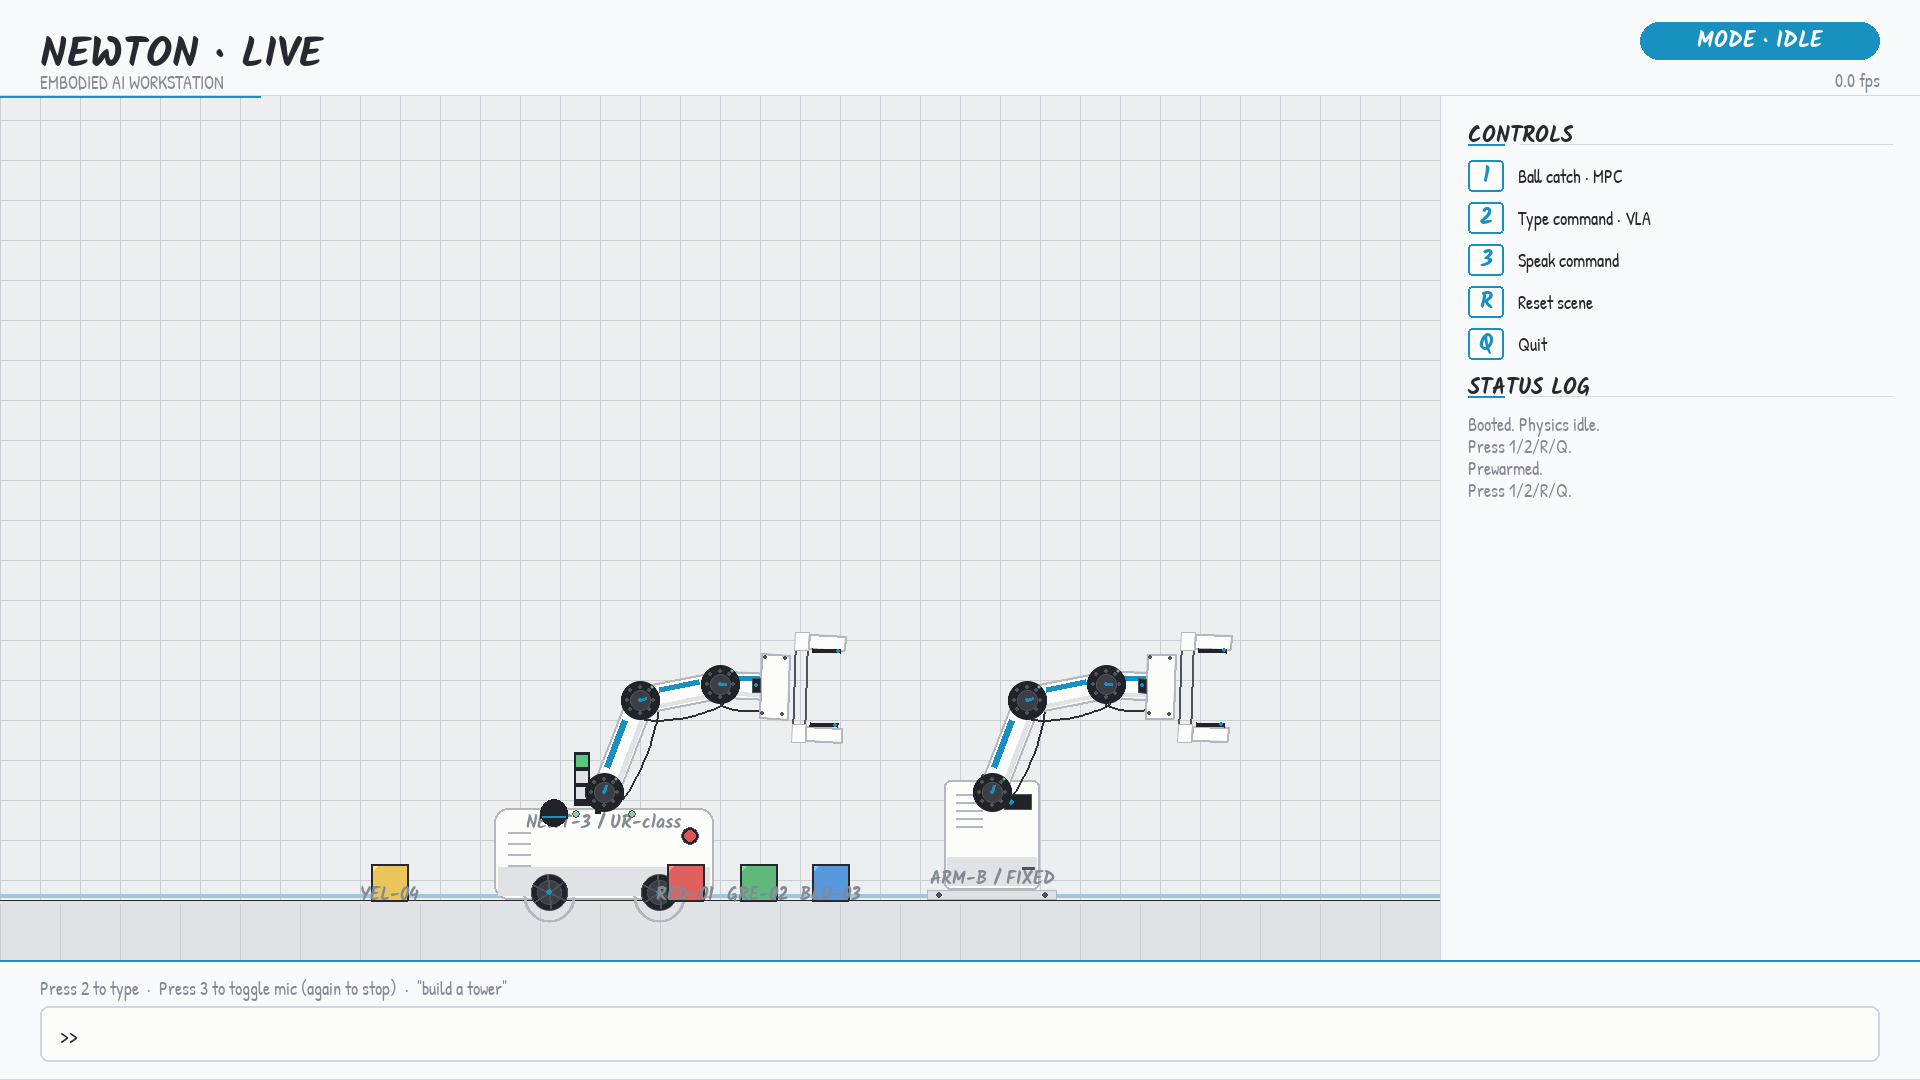
\includegraphics[width=0.82\linewidth]{figures/industrial_view.png}
\caption{IDLE 工业模式：双臂工作站、5 个方块（4 教学色 + 1 灰
workpiece）、侧栏控制提示与状态日志。FPS 计数实时显示。}
\label{fig:industrial}
\end{figure}

\begin{figure}[h]
\centering
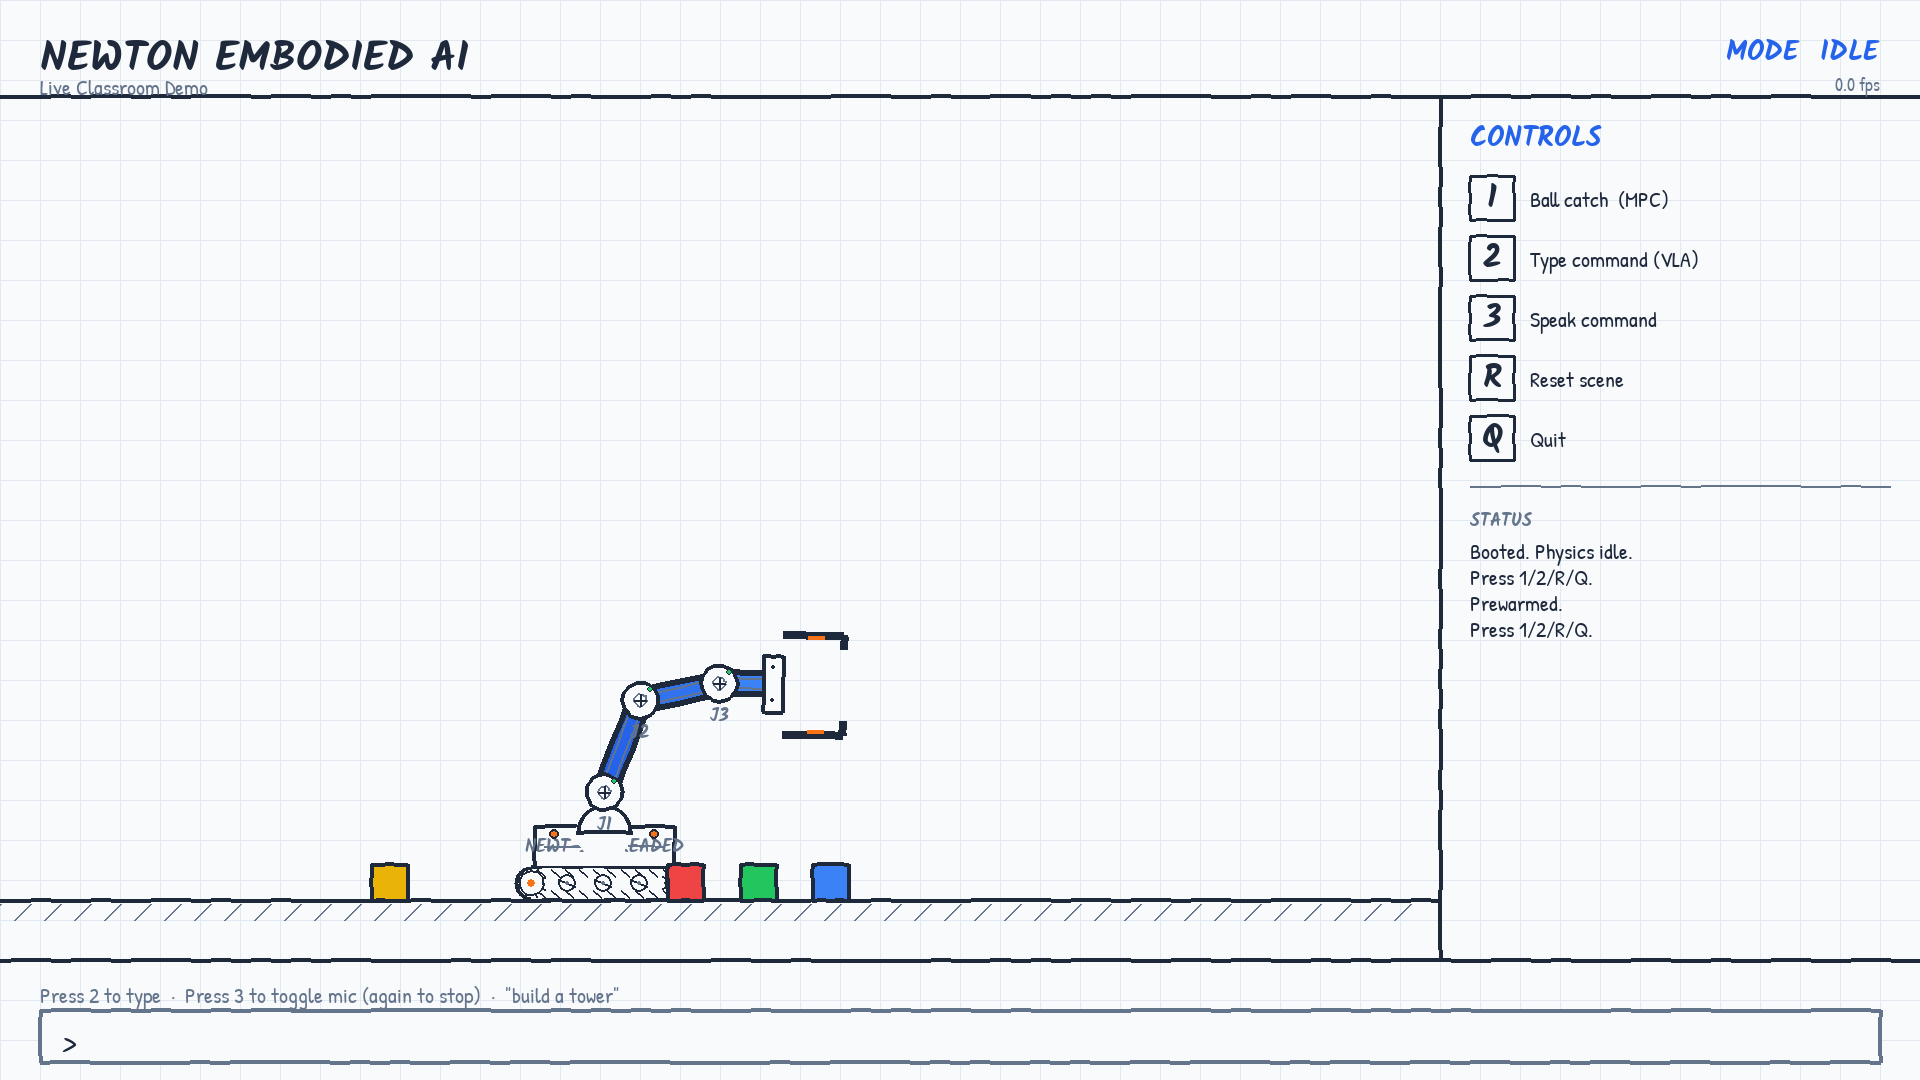
\includegraphics[width=0.82\linewidth]{figures/classroom_view.png}
\caption{IDLE 课堂模式：手绘风格 3-DOF 机械臂、4 教学色方块，
模拟黑板教学场景。无 Arm B。}
\label{fig:classroom}
\end{figure}

\clearpage
\subsubsection{BALL CATCH 模式}
按 \texttt{1} 进入接球模式后，\autoref{fig:catch-industrial}
展示工业模式 ``Tracking'' 状态：
蓝色曲线是小球的实时轨迹采样，橙色圆环是
\texttt{catcher.\_predict()} 计算出的截击点，状态日志连续
打印 \texttt{Caught! (2/2)} 等成功事件。
\autoref{fig:catch-classroom} 是课堂模式的接到后特写——
末端执行器的两指闭合环住小球，状态显示 ``Caught! (3/3)''。

\begin{figure}[h]
\centering
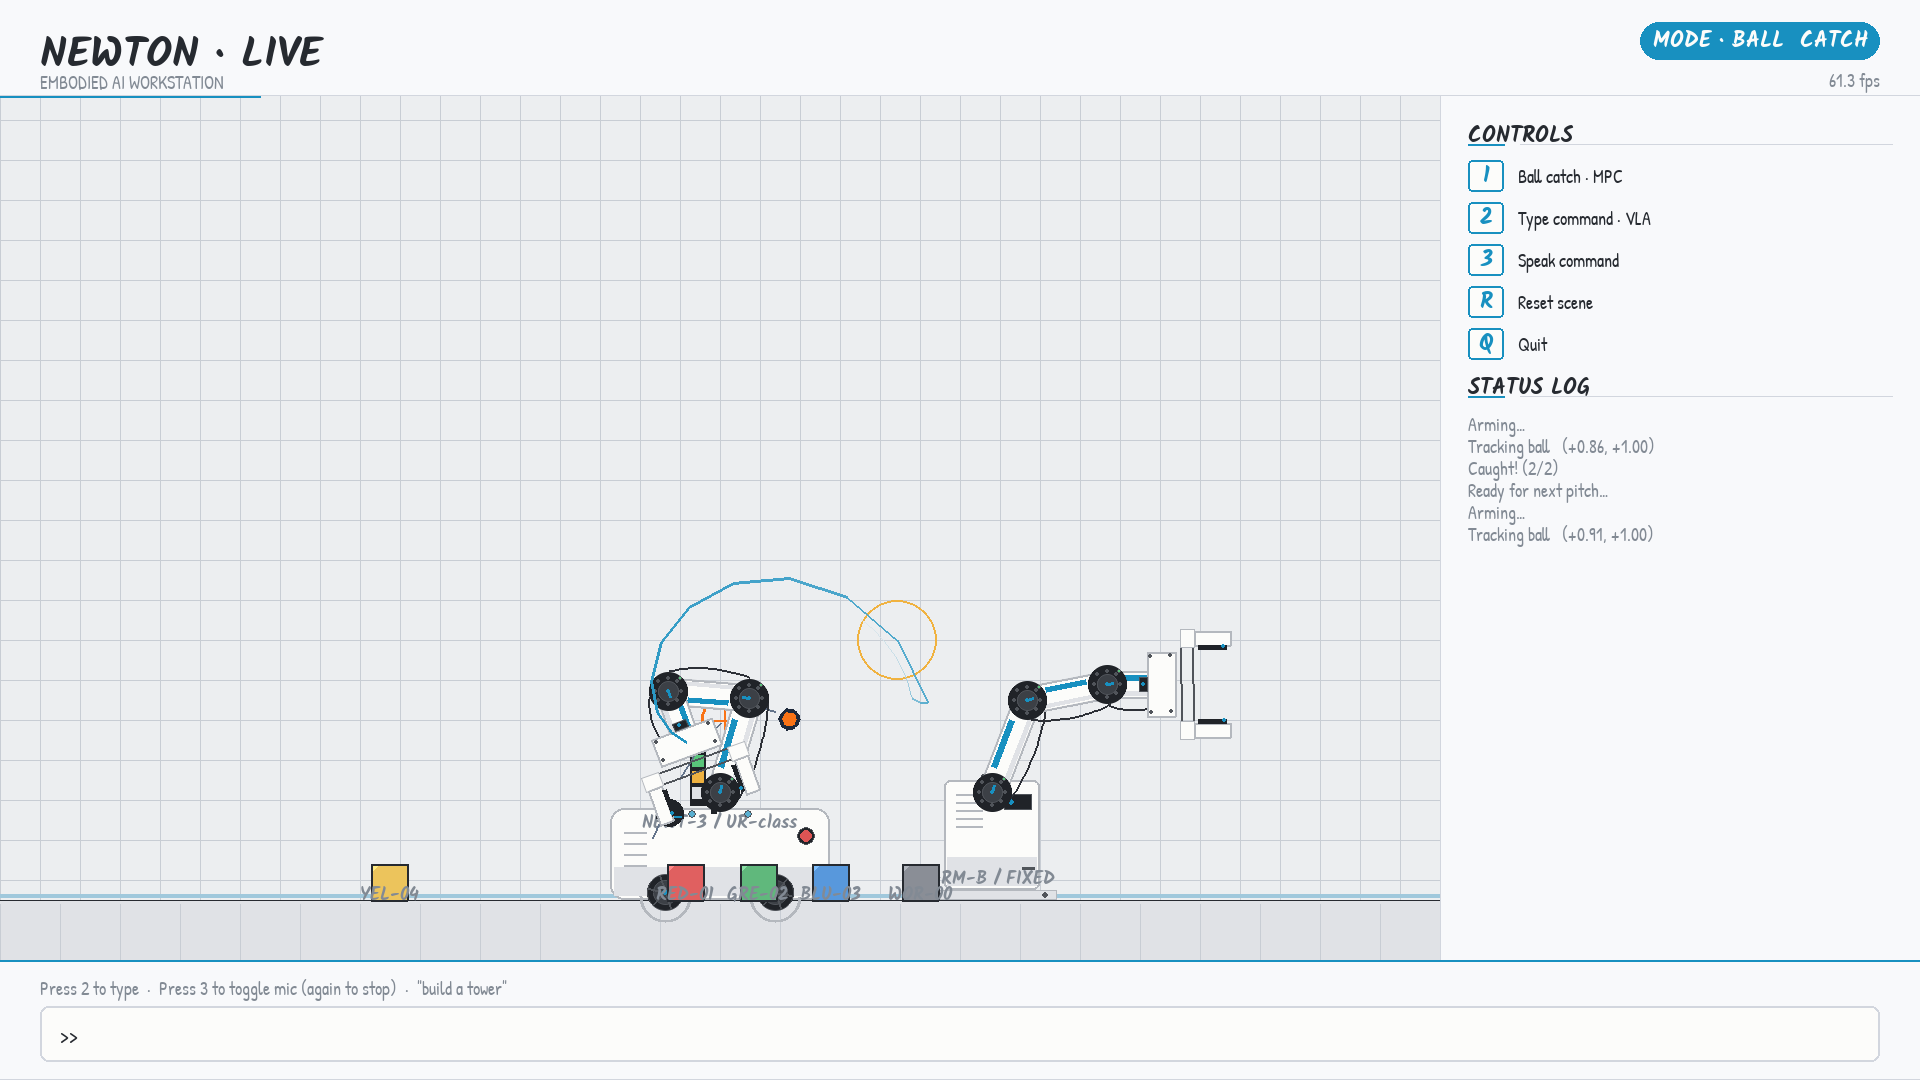
\includegraphics[width=0.82\linewidth]{figures/catch_industrial.png}
\caption{工业模式接球时刻：蓝色轨迹采样 + 橙色截击点圆环，
status log 实时打印追踪坐标。本帧右上 FPS 61.3，下一球
正从右侧飞来。}
\label{fig:catch-industrial}
\end{figure}

\begin{figure}[h]
\centering
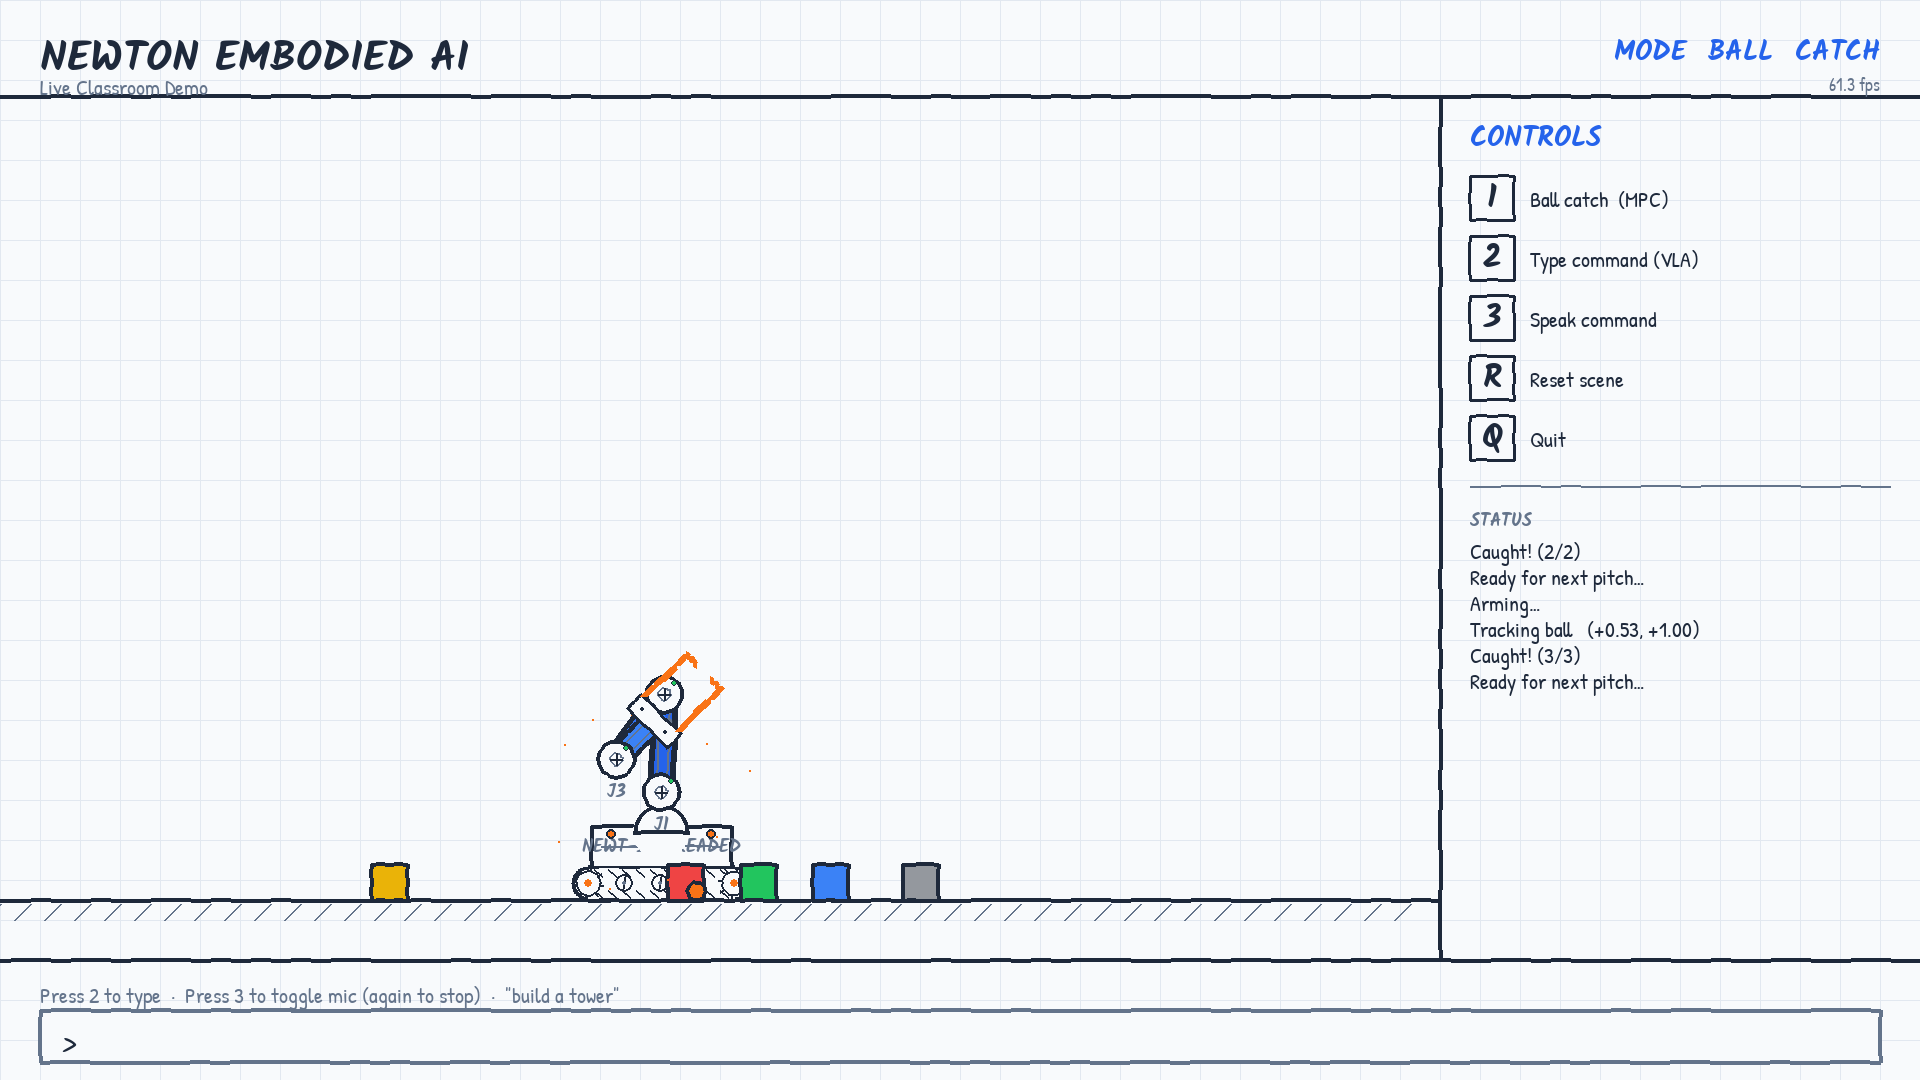
\includegraphics[width=0.82\linewidth]{figures/catch_classroom.png}
\caption{课堂模式接到瞬间：橙色 ``caught'' 高亮包络
小球，状态 ``Caught! (3/3)''。底部有效区显示 5 个静止方块。}
\label{fig:catch-classroom}
\end{figure}

\clearpage
\subsubsection{TASK EXEC 模式}
\autoref{fig:stack-industrial} 是工业模式中 Arm A 执行
\texttt{stack [red, green, blue]} 的中途：手臂正抓住绿块
向左移动，红块已经放置完成；状态日志完整呈现
\texttt{Approach $\to$ Descend + grip $\to$ Picked up
$\to$ Lift $\to$ Driving} 五步流水。
\autoref{fig:stack-classroom} 是课堂模式的塔成型态：
红 + 绿两块已堆好，蓝块即将被放上。

\begin{figure}[h]
\centering
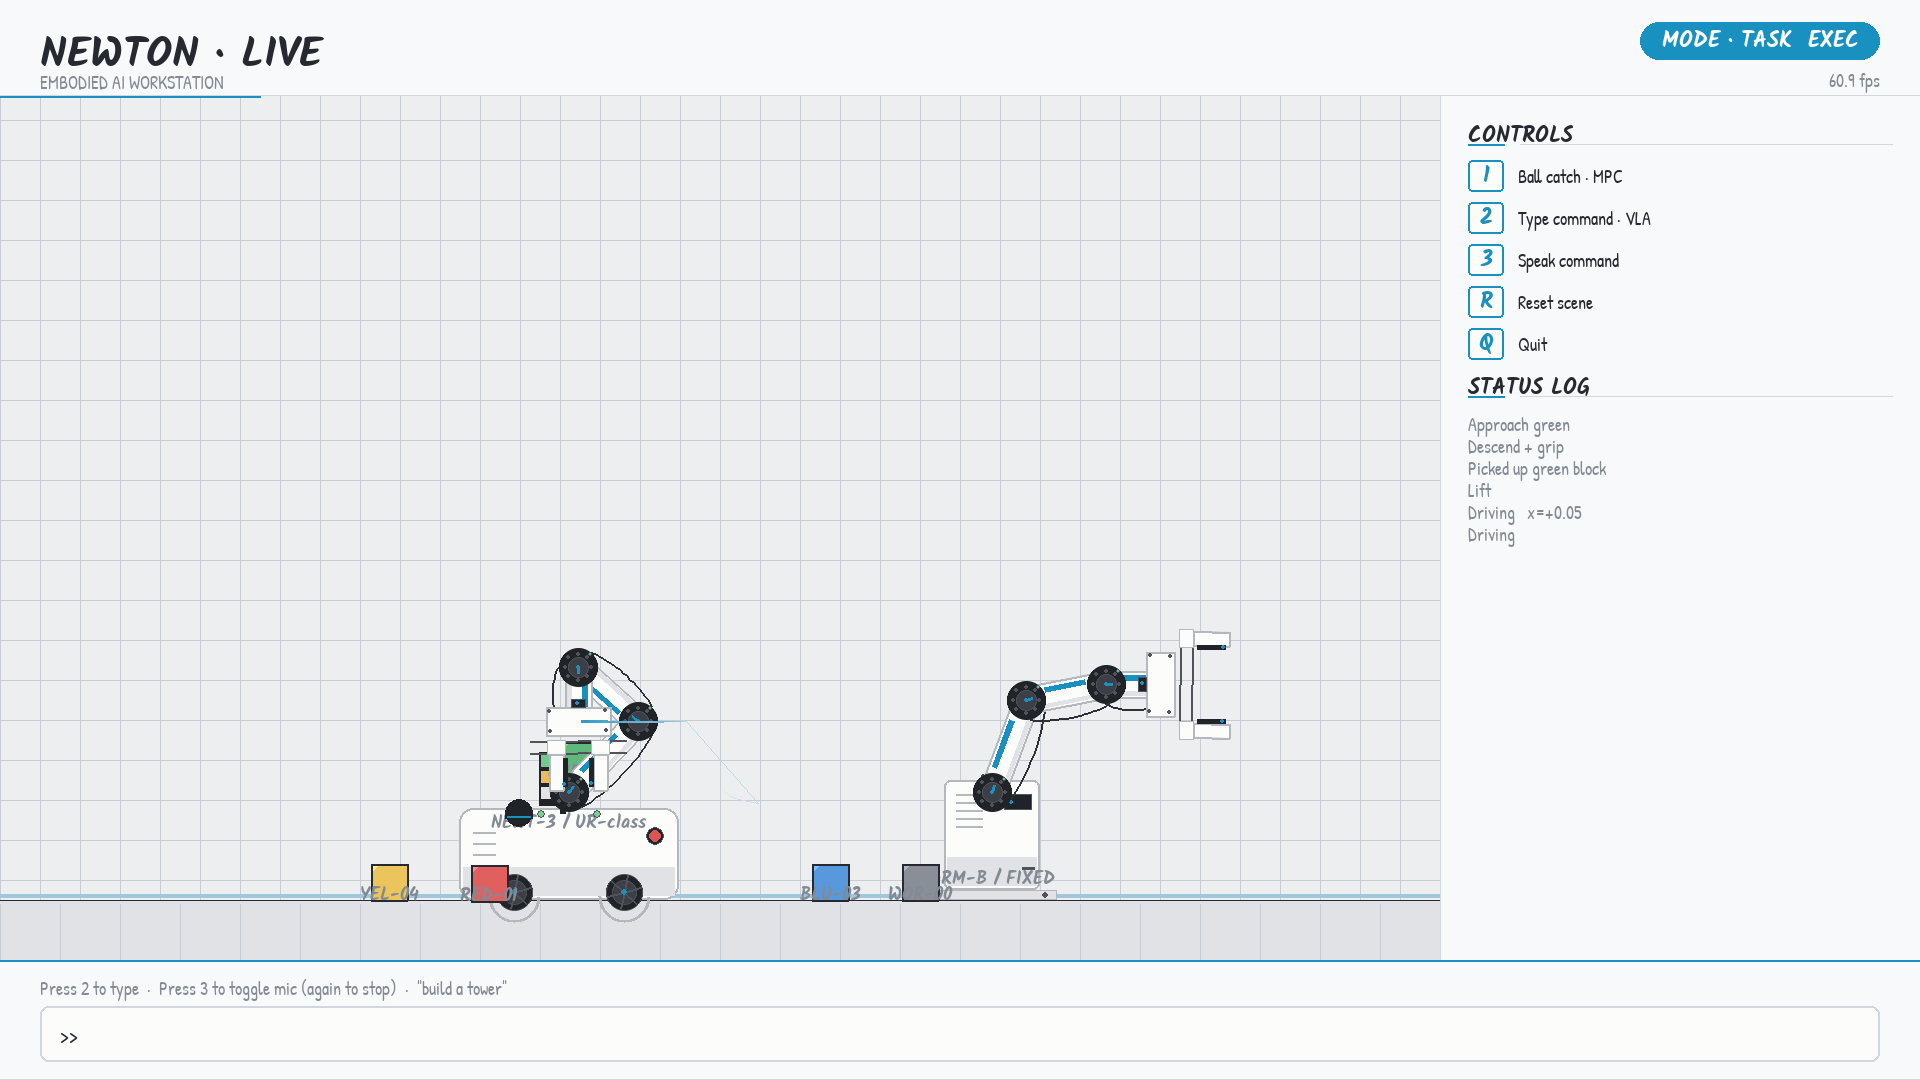
\includegraphics[width=0.82\linewidth]{figures/stack_industrial.png}
\caption{工业模式 \texttt{stack} 执行中：Arm A 持绿块行进，
红块已就位（左下角）。Arm B 闲置在支架上。状态日志逐行
展开\texttt{TaskExecutor} 的 waypoint 推进。}
\label{fig:stack-industrial}
\end{figure}

\begin{figure}[h]
\centering
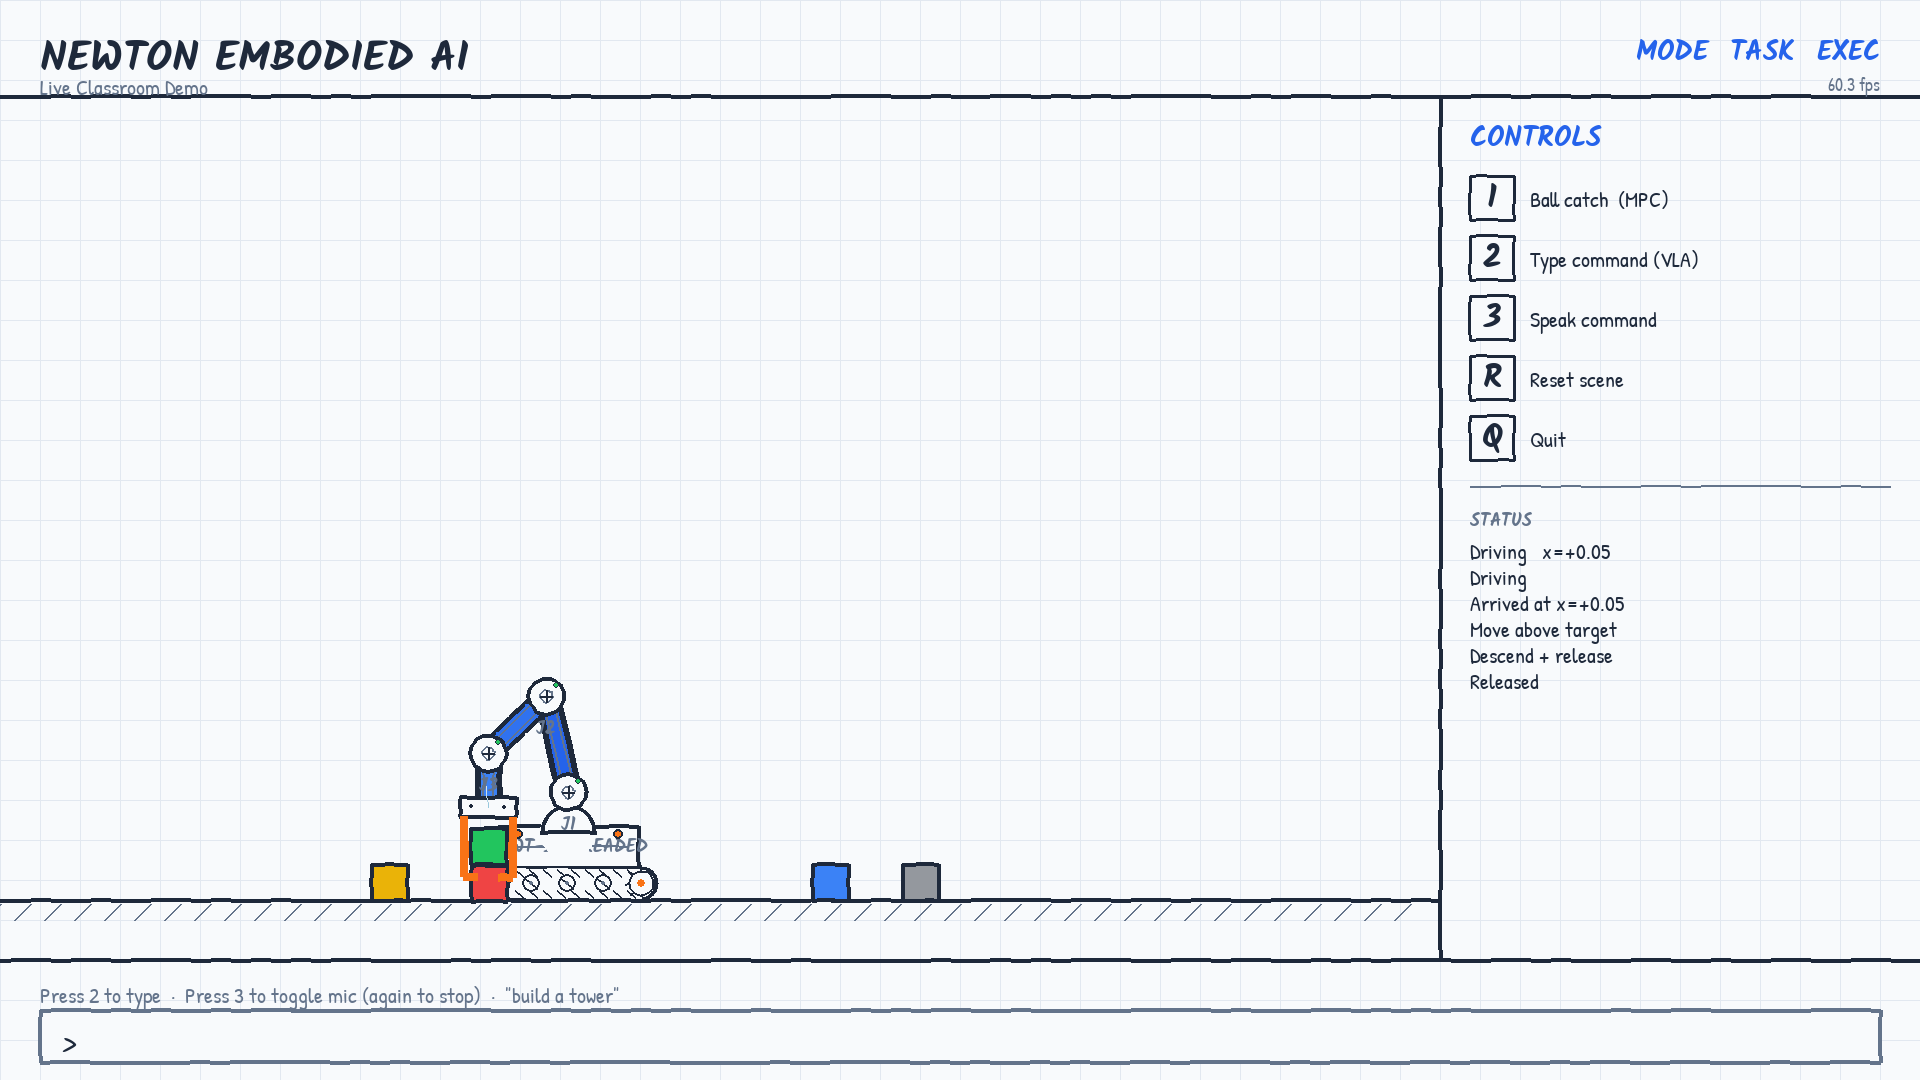
\includegraphics[width=0.82\linewidth]{figures/stack_classroom.png}
\caption{课堂模式 \texttt{stack} 半成型：红块 + 绿块堆好，
蓝块仍在右侧待取。状态日志显示 \texttt{Driving $\to$
Move above $\to$ Descend + release $\to$ Released}。}
\label{fig:stack-classroom}
\end{figure}

\clearpage
\subsubsection{VLA + AI·PARSED 侧栏}
\autoref{fig:vla-panel} 是本演示的``招牌''截图：自然语言
``build a tower of red green and blue'' 经 Claude 解析后，
\textbf{AI · PARSED} 侧栏完整展开 7 个字段——
\texttt{user}, \texttt{via} (\texttt{claude 9564ms}),
\texttt{action} (\texttt{stack}),
\texttt{colors} (\texttt{['red','green','blue']}),
\texttt{reason} (\texttt{build tower with red, green, blue})。
status log 显示 \texttt{via Claude confirmed (9564ms)}
这一关键事件，证实混合管线工作正常。本帧 Arm A 已堆好
红 + 绿两块，正持蓝块行进中。

\begin{figure}[h]
\centering

\includegraphics[width=0.92\linewidth]{figures/vla_panel_industrial.png}
\caption{VLA 推理迹侧栏。用户输入 + Claude 后端 + 9564 ms
延迟 + 解析后的结构化动作全部可见，观众能直接看到
``AI 在想什么''。这是 D.1 的核心交付。}
\label{fig:vla-panel}
\end{figure}

% ============================================================
\section{总结与展望}\label{sec:conclusion}

\subsection{已完成工作}
\begin{itemize}[leftmargin=*, itemsep=0pt]
  \item 三模式交互演示：接球 (MPC)、自然语言 (VLA)、手势；
  \item 双渲染管线：课堂白板 + 工业双臂工作站；
  \item 混合 VLA 解析：preflight $1$\,ms + Claude 后台精化；
  \item Arm B 自主工件搬运循环；
  \item 214 项自动化测试，60 fps 稳定，实战命中 62\%--82\%；
  \item 完整 CSV 遥测 + 公式注入防护；
  \item 文档同步：README + REHEARSAL 与代码 100\% 一致。
\end{itemize}

\subsection{局限性}
\begin{enumerate}[leftmargin=*]
  \item \texttt{\_\_main\_\_.py} 仍有 1139 行，超出项目编码
    规范的 800 行硬上限。完整 AppState dataclass 重构需要
    架构改动，本项目阶段性接受这一债务；
  \item D.3 慢动作是简化版 (整体放慢 dt)，原计划的逐帧
    snapshot replay 因实现复杂度被降级；
  \item 语音模糊匹配仅覆盖 en-US / zh-CN，未扩展到日韩等
    语言；
  \item 接球 MPC 是单步式（每帧重拟合，无前瞻规划），
    复杂多轨道场景下精度有限。
\end{enumerate}

\subsection{未来工作}
\begin{itemize}[leftmargin=*, itemsep=0pt]
  \item \textbf{AppState 重构}：定义可变 dataclass 收纳全部
    主循环状态，把 \texttt{\_\_main\_\_.py} 切到 $\leq 200$
    行；
  \item \textbf{完整逐帧 replay}：环形缓冲器 + 渲染层 source
    切换，比 slow-mo 更具戏剧化；
  \item \textbf{多臂协调}：Arm B 检测 Arm A 持物时让出工作区，
    更接近真实工厂调度；
  \item \textbf{多语言扩展}：日语 / 韩语 / 西语模糊匹配 +
    Claude prompt 本地化。
\end{itemize}

% ============================================================
\section*{致谢}
感谢 NVIDIA 开源 Newton 物理引擎，为本演示提供了高品质的
仿真后端。感谢 Anthropic 的 Claude 命令行客户端，让自然
语言驱动机器人成为本地可行的方案。

% ============================================================
\begin{thebibliography}{9}

\bibitem{newton}
NVIDIA, ``Newton: A GPU-accelerated, differentiable physics engine,''
\url{https://github.com/newton-physics/newton}, 2025.

\bibitem{xpbd}
Macklin, M., Müller, M., Chentanez, N., ``XPBD: position-based
simulation of compliant constrained dynamics,''
\textit{Proc. ACM MIG}, 2016.

\bibitem{anthropic}
Anthropic, ``Claude Code: A CLI for agentic coding,''
\url{https://claude.com/claude-code}, 2025.

\bibitem{minjerk}
Flash, T., Hogan, N., ``The coordination of arm movements: an
experimentally confirmed mathematical model,''
\textit{J. Neuroscience}, vol.\,5, no.\,7, pp.\,1688--1703, 1985.

\bibitem{ik}
Murray, R.M., Li, Z., Sastry, S.S., ``A Mathematical Introduction
to Robotic Manipulation,'' CRC Press, 1994.

\bibitem{vla}
Brohan, A. et al., ``RT-2: Vision-Language-Action Models Transfer
Web Knowledge to Robotic Control,'' arXiv:2307.15818, 2023.

\bibitem{speech}
Google, ``Cloud Speech-to-Text,''
\url{https://cloud.google.com/speech-to-text}.

\end{thebibliography}

\end{document}
